\section{BP on a grid}
\label{app:bp}

\note{Grid, trapezoid weights, kernel matrix, the two sweeps, posterior mean, pair posteriors, log-likelihood from the
forward normalisers, cost.}

\label{app:numerics}
\begin{figure}[h]
  \centering
  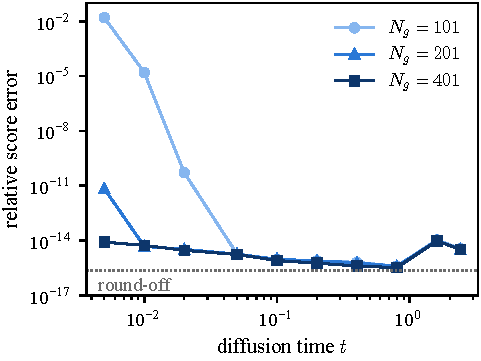
\includegraphics{fig_grid_gaussian}\hfill
  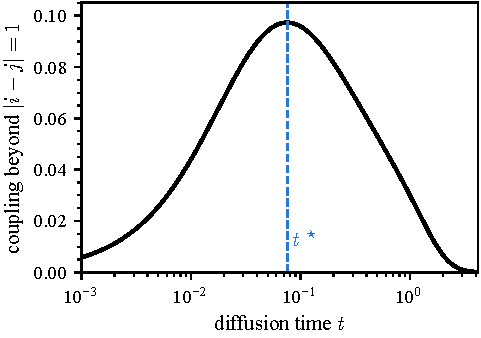
\includegraphics{fig_locality_curve}
  \caption{\note{Left: grid BP against $-Q_tx$, Gaussian chain, $N_g=101$, $201$, $401$ (round-off for
  $t\geq0.05$). Right: coupling of $Q_t$ beyond nearest neighbours against $t$, peak at $t^\star$.}}
  \label{fig:grid}
\end{figure}

\section{EM: M-steps}
\label{app:em}

\note{Closed forms (Gaussian and Laplace AR(1)), mixture ECM, log-linear (concave, observed minus expected), neural
(autograd on $Q$, GEM). Checkpoint ladder and selection.}

\begin{figure}[h]
  \centering
  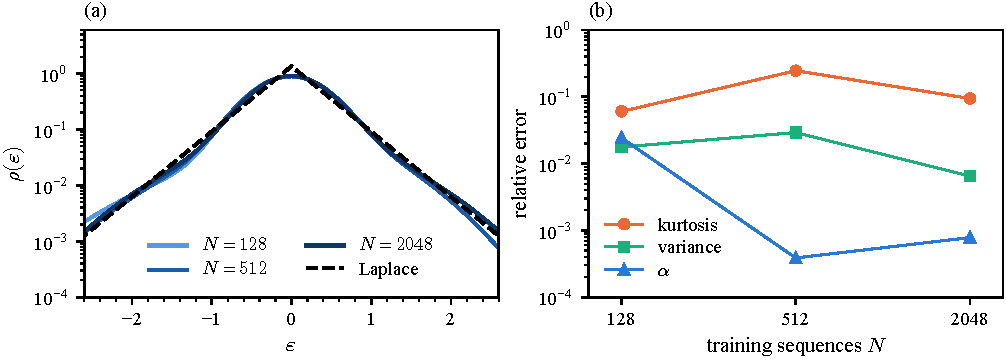
\includegraphics{fig_em_innovation}
  \caption{\note{Mixture ($C=8$): learned innovation law, and relative error of $\alpha$, variance and kurtosis
  against $N$ (thesis Fig.~6.3).}}
  \label{fig:em-innovation}
\end{figure}

\section{Sources of error}
\label{app:errors}

\note{J\'er\^ome (20:14): the error decomposition is ``typical appendix stuff''. Grid, misspecification, finite data,
EM stopping.}

\section{Network baselines}
\label{app:networks}

\note{Architectures and parameter counts (MLP 26{,}016, CNN 5{,}505, BiGRU 15{,}169), screen, recipe, pairing.}

\section{Allen--Cahn details}
\label{app:field}

\note{Cells, families, networks, the $M=128$ table (slide-15 note).}
